\documentclass{article}
\usepackage[utf8]{inputenc}
\parskip = 0.75em
\parindent = 10mm
\def\baselinestretch{1}
\usepackage {float}
\usepackage{listings}
\usepackage{subcaption}
\usepackage[usenames]{color}
\usepackage[numbers,sort&compress]{natbib}
\usepackage{multirow, array}
\usepackage[spanish]{babel}
	\deactivatetilden
	\spanishdecimal{.}
	\addto\captionsspanish{\def\tablename{Tabla}}
	\addto\captionsspanish{\def\listtablename{\'Indice de tablas}}

\usepackage{amsmath,amsfonts,amssymb}
	\allowdisplaybreaks[4]
\usepackage{graphicx}
	\graphicspath{{Figuras/}}
\usepackage[clearempty,pagestyles]{titlesec}
\usepackage{anysize}

\def\baselinestretch{1.5}
\papersize{27.9cm}{21.5cm} 
\marginsize{2cm}{2cm}{1cm}{1cm}

\begin{document}


	\begin{center}
	\huge{\textbf{Tarea 11 Frentes de Pareto}}\\
	
	\textsc{ \Large Susana Ruiz Nuñez}
	\end{center}


\section{Planteamiento del problema} 
En esta práctica \cite{satu} se estudia como parte de la optimización multicriterio, un mismo conjunto de variables que ocupan asignarse valores de tal forma que se optimizen dos o más funciones objetivos que pueden contradecir una a otra teniendo en cuenta un número determinado de restricciones. Aparece el término de dominancia de Pareto donde una solución domina a otra si no empeora ninguno de los objetivos y mejora a por lo menos uno. 

\section{Metodología}
Para el desarrollo de esta práctica se necesita graficar el porcentaje de soluciones Pareto como función del número de funciones objetivo para $k \in [2, 12, 2]$ (por limitaciones del equipo se hizo para las funciones pares) en una combinación de diagrama de violín y caja-bigote. Se crea una función para la repetición de un total de 25 iteraciones y para las funciones pares entre los valores dos y doce con 250 soluciones aleatorias. Se crea una variable para hallar el porcentaje de los valores no dominados, también conocido como frente Pareto. Se muestra una parte del resultado del experimento.  

\begin{lstlisting}[language=Python]
			Funcion Objetivo  Porciento Pareto
		0                 02               3.6
		1                 02               5.6
		2                 02               1.2
	
		25                04               3.6
		26                04              46.0
	
		50                06              52.8
		51                06              43.2
	
		75                08              99.6
		76                08              78.4
	
		100               10             100.0
		101               10              70.8
	
		125               12              99.2
		126               12             100.0
\end{lstlisting}


\section{Resultados y razonamiento escrito}

Los resultados que muestra la gráfica exponen que para solo dos funciones el porciento de valores no dominados o frente Pareto es muy bajo, rozando valores cercanos a cero. Al aumentar a cuatro y seis funciones se ve un comportamiento donde son amplios los porcientos de valores no dominados y su influencia sobres los valores dominados es bastante constante. Para el número de funciones ocho se muestra otro comportamiento diferente a lo visto hasta el momento; los valores no dominados comienzan a ser mayores con respecto al total de valores. Este comportamiento de agudiza para cuando hay diez y doce funciones, llegando en esta última a ser casi la totalidad de valores los no dominados. Esto se debe a que al aumentar el número de funciones que inciden una sobre otra, se va haciendo más pequeño el número de soluciones posibles que mejore una función y empeore la otra. Se va haciendo el cerco más reducido por así decirlo.


\begin{figure}[H]
\centering
	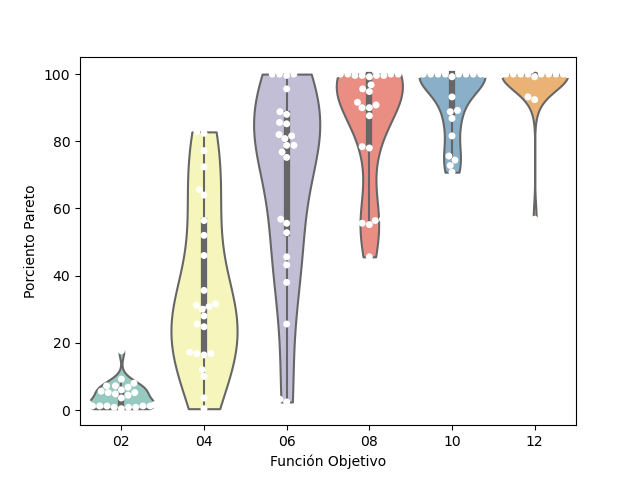
\includegraphics[scale=0.8]{Figure_1.png}
	\caption{Porciento del frente Pareto para diferentes números de funciones objetivos.}
	\label{1}		
\end{figure}



\section{Conclusiones}
Se concluye con los experimentos realizados que los frentes de Pareto son de gran utilidad en la vida cotidiana, en experimentos, en el sector empresarial cuando se quiere analizar el comportamiento de una característica con la influencia de otra.

\bibliography{Tarea11}
\bibliographystyle{plainnat}
\end{document} 
